\documentclass[a4paper, 12pt]{article}

% Для многоязычности
\usepackage{polyglossia}
\setdefaultlanguage[indentfirst=true,spelling=modern]{russian}
\setotherlanguage{english}
% Юникодные математические символы
\usepackage{unicode-math}

\usepackage{amsmath}

\usepackage{fontspec}
% Подключаем шрифт. Шрифт есть в дистрибутиве TeXLive
\setmainfont[Ligatures={Common,TeX},Scale=0.94]{IBM Plex Serif}
\setromanfont[Ligatures={Common,TeX},Scale=0.94]{IBM Plex Serif}
\setsansfont[Ligatures={Common,TeX},Scale=MatchLowercase,Scale=0.94]{IBM Plex Sans}
\setmonofont[Scale=MatchLowercase,Scale=0.94,FakeStretch=0.9]{IBM Plex Mono}

% Математический шрифт
\setmathfont{STIX Two Math}

\usepackage{setspace}
\onehalfspacing

\usepackage[backend=biber,sorting=none]{biblatex}
\addbibresource{bib/cite.bib}

% Пакет для подключения картинок
\usepackage{graphicx}
% Пакет для ссылок (hyper references)
\usepackage[hidelinks]{hyperref}

\usepackage{listings}
\usepackage{xcolor}
\usepackage{caption}
% Настройка листингов кода
\lstdefinestyle{mystyle}{
    backgroundcolor=\color{black!5},
    commentstyle=\color{green!40!black},
    keywordstyle=\color{blue},
    stringstyle=\color{purple},
    basicstyle=\footnotesize\ttfamily,
    numbers=left,
    breaklines=true,
    numberstyle=\tiny\color{black!60},
    frame=tb,
    framerule=0pt,
    keepspaces=true,
}
\lstset{style=mystyle}

\usepackage{float}
\usepackage{lipsum} % Для генерации текста-"рыбы"


\renewcommand{\figurename}{Рис.}
\renewcommand{\tablename}{Таблица}
\renewcommand{\lstlistingname}{Листинг}
\renewcommand{\contentsname}{Содержание}
\renewcommand{\listfigurename}{Список иллюстраций}
\renewcommand{\listtablename}{Список таблиц}
\renewcommand{\lstlistlistingname}{Список листингов}

\usepackage{geometry}
\geometry{left=2.5cm, right=1.5cm, top=2cm, bottom=2cm}

\author{Николаев Дмитрий Иванович, НПМмд-02-24}
\title{Лабораторная работа №8: Создание диаграмм и рисунков с помощью TikZ в \LaTeX \\ Computer Skills for Scientific Writing}
\date{\today}

\begin{document}
  \maketitle
  \tableofcontents
  \pagebreak

  \listoffigures
  \lstlistoflistings
  \pagebreak

\section{Цель работы}
Целью данной работы является доскональное изучение и практическое освоение инструментов создания векторной графики в \LaTeX\ с использованием пакета TikZ. Задача включает в себя воспроизведение примеров построения примитивов, графов, графиков функций и фрактальных структур из учебного пособия~\cite{lab}, а также выполнение итоговых упражнений на создание сложных иллюстраций.

\section{Теоретическое введение}
Пакет TikZ (рекурсивный акроним от нем. \textit{TikZ ist kein Zeichenprogramm} --- «TikZ --- это не программа для рисования») представляет собой мощный инструмент для создания графики программным путем непосредственно в коде \LaTeX. В отличие от визуальных редакторов, TikZ позволяет описывать изображения с помощью команд, что обеспечивает высочайшее качество печати, единый стиль с основным документом (шрифты, математические формулы) и возможность автоматизации.

Рисунки создаются внутри окружения \texttt{tikzpicture}. Основными строительными блоками являются пути (paths), узлы (nodes) и стили. TikZ поддерживает декартовы и полярные координаты, циклы \texttt{\textbackslash foreach}, математические вычисления (через библиотеку \texttt{tikz.math}) и множество библиотек для специфических задач (графы, цепи, диаграммы).

\section{Выполнение лабораторной работы}
Были последовательно воспроизведены все примеры из раздела 8 «Diagrams and drawings as code» учебного пособия~\cite{lab}, после чего выполнены задания для самостоятельной работы.

\subsection{Часть 1: Воспроизведение примеров из пособия}

\paragraph{1.1. Рисование прямых линий.}
Первым шагом было освоение команды \texttt{\textbackslash draw}. Координаты задаются в круглых скобках (x,y) или в полярной системе (угол:длина). Код приведён в \lstlistingname~\ref{lst:lines}, результат --- на \figurename~\ref{fig:001}.

\begin{lstlisting}[float=htbp, language=tex, caption={Базовое рисование линий}, label=lst:lines]
\begin{tikzpicture}
    \draw (-1,0) -- (3,10pt) -- (35:3);
\end{tikzpicture}
\end{lstlisting}

\begin{figure}[H]
\centering
% Здесь должен быть скриншот результата
\includegraphics[width=0.5\textwidth]{image/1.png}
\caption{Результат рисования ломаной линии по координатам}
\label{fig:001}
\end{figure}

\paragraph{1.2. Стилизация линий и кривые.}
Далее были рассмотрены опции стилизации (стрелки \texttt{->}, цвет \texttt{red}) и специальные типы соединений: ортогональные сегменты (\texttt{-|}) и кривые линии с использованием команд \texttt{to[out=..,in=..]} и кривых Безье через \texttt{.. controls ..}.

\begin{lstlisting}[float=htbp, language=tex, caption={Стилизация линий и кривые Безье}, label=lst:curves]
\begin{tikzpicture}
    \draw[->] (-1,0) -| (3,10pt);
    \draw[red] (3,10pt) -- (35:3);
\end{tikzpicture}

\begin{tikzpicture}
    \draw (-1,0) to (5,1);
    \draw[green] (-1,0) to[out=90,in=135] (5,1);
    \draw[cyan] (-1,0) .. controls (0,-2) .. (5,1);
\end{tikzpicture}

\begin{tikzpicture}
    \draw[dotted,gray] (-1,0) -- (5,1);
    \draw (-1,0) .. controls (0,-2) and (4,2) .. (5,1);
\end{tikzpicture}
\end{lstlisting}

\begin{figure}[H]
\centering
\includegraphics[width=0.7\textwidth]{image/2.png}
\caption{Различные типы линий и кривых}
\label{fig:002}
\end{figure}

\paragraph{1.3. Узлы (Nodes).}
Узлы используются для добавления текста и меток. Рассмотрено размещение узлов относительно координат и линий с помощью опций \texttt{midway}, \texttt{pos}, \texttt{above}, \texttt{right}.

\begin{lstlisting}[float=htbp, language=tex, caption={Размещение текстовых узлов}, label=lst:nodes]
\begin{tikzpicture}[scale=3]
\draw (0,0) node {hello} -- (1,1) node {world};
\end{tikzpicture}

\begin{tikzpicture}[scale=3]
\draw (0,0) -- (1,1) node[midway]{A} node[pos=0.75,above]{B} node[below right]{C};
\end{tikzpicture}

\begin{tikzpicture}[scale=3]
\draw (0,0) to node[midway]{A} node[pos=0.75, above]{B} (1,1) node[right]{C};
\end{tikzpicture}
\end{lstlisting}

\begin{figure}[H]
\centering
\includegraphics[width=0.6\textwidth]{image/3.png}
\caption{Примеры размещения текстовых меток (узлов)}
\label{fig:003}
\end{figure}

\paragraph{1.4. Узлы с формулами и фигурами.}
Узлы могут содержать математические формулы и иметь форму (круг, прямоугольник), если задана опция \texttt{draw}. Также была изучена техника именования узлов для последующего соединения их линиями.

\begin{lstlisting}[float=htbp, language=tex, caption={Узлы с оформлением и математикой}, label=lst:mathnodes]
\begin{tikzpicture}[scale=3]
\draw (0,0) node[circle, draw]{$\sum\limits_{i=1}^{n}n^2$} -- (1,1)
node[rectangle,draw]{$\frac{1}{\sqrt{2}}$};
\end{tikzpicture}

\begin{tikzpicture}[scale=3]
% define nodes
\node[circle,draw] (label1) at (0,0) {$\sum_{i=1}^{n}n^2$};
\node[rectangle,draw] (label2) at (1,1) {$\frac{1}{\sqrt{2}}$};
% draw the line
\draw (label1) -- (label2);
\end{tikzpicture}
\end{lstlisting}

\begin{figure}[H]
\centering
\includegraphics[width=0.5\textwidth]{image/4.png}
\caption{Соединенные узлы с математическим содержимым}
\label{fig:004}
\end{figure}

\paragraph{1.5. Сложный граф.}
Итоговый пример первой части демонстрирует объединение всех техник: определение именованных узлов разной формы и цвета, и соединение их различными типами линий (пунктирными, кривыми, цветными) с подписями.

\begin{lstlisting}[float=htbp, language=tex, caption={Построение сложного графа}, label=lst:complexgraph]
\begin{tikzpicture}[scale=2]
% Define the nodes
\node[circle, draw] at (0,0) (a) {A};
\node[rectangle, fill] at (3,0) (b) {};
\node at (3,0.4) (blabel) {B};
\node[rectangle,rounded corners, draw] at (5,2) (c) {C};
% Draw the paths
\draw[->, green] (a) -- (b) node[midway, below,black]{2};
\draw[<->, blue] (a) to[out=45, in=135] (b);
\draw[->,red] (b)--(c);
\draw[brown,dotted,very thick] (b) |- (c);
\draw[<-,cyan] (b) -| (c);
\draw[thick,black] (a).. controls (1,5) .. (c) node[midway, above]{$\frac{1}{2}$};
\end{tikzpicture}
\end{lstlisting}

\begin{figure}[H]
\centering
\includegraphics[width=0.7\textwidth]{image/5.png}
\caption{Сложный граф, объединяющий разные техники TikZ}
\label{fig:005}
\end{figure}

\paragraph{1.6. Графики функций и циклы.}
TikZ позволяет строить графики элементарных функций, указывая домен (область определения) и количество точек выборки (\texttt{samples}). Также изучены циклы \texttt{\textbackslash foreach} для повторяющихся действий.

\begin{lstlisting}[float=htbp, language=tex, caption={График параболы, косинуса и циклы}, label=lst:plots]
\begin{tikzpicture}
\draw [domain=-2:2] plot (\x, {pow(\x,2});
\end{tikzpicture}

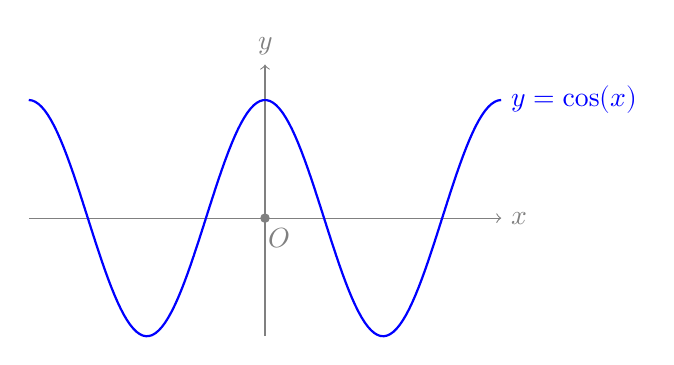
\begin{tikzpicture}[scale=1.5]
% Draw the x and y axis, label the axes and the origin
\draw[gray, ->] (-2,0) -- (2,0) node[right]{$x$} node[pos=0.53, below]{$O$};
\draw[gray, ->] (0,-1) -- (0,1.3) node[above]{$y$};
\draw[fill,gray] (0,0) circle [radius=1pt];
% Plot the curve
\draw[blue, thick] [domain=-2:2, samples=150] plot (\x, {cos(pi*\x r)}) node[right]{$y = \cos(x)$};
% Note: the r in the argument of the cosine signifies that we enter \x in radians
\end{tikzpicture}

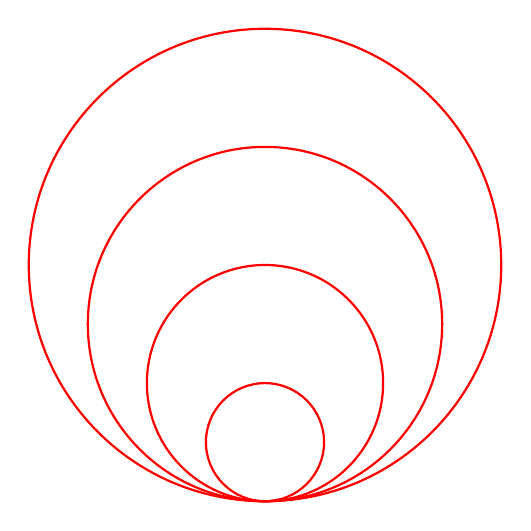
\begin{tikzpicture}[scale=0.75]
\foreach \x in {0,1,2,3}
\draw[red,thick] (0,\x) circle [radius=\x+1];
\end{tikzpicture}
\end{lstlisting}

\begin{figure}[H]
\centering
\includegraphics[width=0.8\textwidth]{image/6.png}
\caption{График функции $y = x^2$, $y=\cos(x)$ и концентрические окружности}
\label{fig:006}
\end{figure}

\paragraph{1.7. Фракталы (Треугольник Серпинского).}
С использованием библиотеки \texttt{tikz.math} была реализована рекурсивная функция для построения треугольника Серпинского.

\begin{lstlisting}[float=htbp, language=tex, caption={Треугольник Серпинсокго}, label=lst:sierpinski_triangle]
\usepackage{tikz}
\usetikzlibrary{math}

% Define a equilateral triangle with lower left corner at coordinate #1 and
% with length of the sides #2
\newcommand\Triangle[2]{
	\draw #1 coordinate(a) -- ++(0:#2) coordinate(b);
	\draw (a) -- ++(60:#2) coordinate(c);
	\fill (a) -- (b) -- (c) -- cycle;
}

\begin{document}
\begin{tikzpicture}
	\tikzmath{
		% Define the recursive function sierpinski
		function sierpinski(\x, \y, \s, \d) {
			if (\d == 0) then {
				% Draw a triangle lower left corner at (\x, \y), length \s 
				{ \Triangle{(\x,\y)}{\s}; };
			} else {
				% Rescale the length of the sides and choose correct coords
				% for the next triangles
				\u1 = 0.25*\s;
				\u2 = \u1*sqrt(3);
				\u3 = 0.5*\s;
				sierpinski(\x,\y,\u3,\d-1);
				sierpinski(\x+\u3,\y,\u3,\d-1);
				sierpinski(\x+\u1,\y+\u2,\u3,\d-1);
			};
		};
		% Let the length of the sides of the base triangle be 4, and generate 6 figures
		\S = 4;
		for \d in {0,...,5}{
			% To situate all plots nicely under and next to each other, define the coords
			% of the lower left corners preemptively
			\x = (\S+1)*mod(\d,2);
			\y = int(\d/2) * (\S+1);
			sierpinski(\x,-\y,\S,\d);
			};
		}
\end{tikzpicture}
\end{lstlisting}

\begin{figure}[H]
\centering
\includegraphics[width=0.9\textwidth]{image/7.png}
\caption{Итерации треугольника Серпинского}
\label{fig:007}
\end{figure}

\subsection{Часть 2: Итоговые упражнения}

\paragraph{2.1. Упражнение 1: Граф с полярными координатами.}
Необходимо было построить граф с 6 узлами по кругу. Использовались полярные координаты (угол:радиус) для размещения узлов A--F.

\begin{lstlisting}[float=htbp, language=tex, caption={Код для Упражнения 1 (Граф)}, label=lst:ex1]
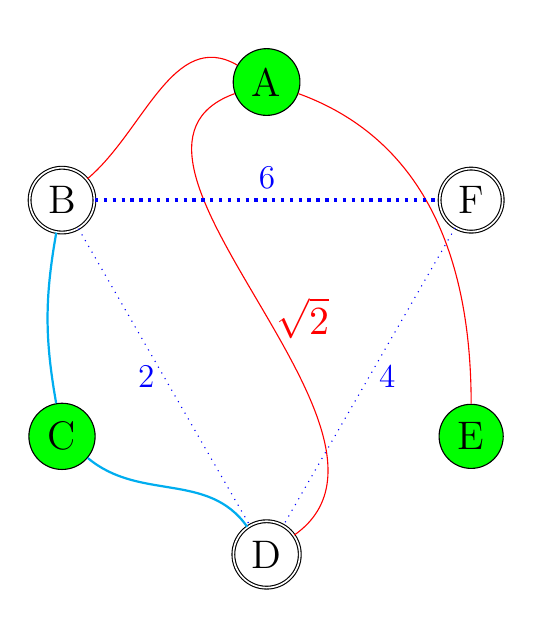
\begin{tikzpicture}
    % Определение узлов в цикле
    \foreach \angle/\label/\col in {150/B/white, 270/D/white, 30/F/white} {
        \node[circle, draw, double, fill=\col, minimum size=0.8cm] (\label) at (\angle:3cm) {\Large \label};
    }
    \foreach \angle/\label/\col in {90/A/green, 210/C/green, 330/E/green} {
        \node[circle, draw, fill=\col, minimum size=0.8cm] (\label) at (\angle:3cm) {\Large \label};
    }
    
    % Соединения
    \draw[red] (A) to[out=150, in=40] (B);
    \draw[red] (A) to[out=200, in=35] (D) node[midway, right] {\Large $\sqrt{2}$}; % Кривая sqrt(2)
    \draw[red] (A) to[out=340, in=90] (E);
    
    \draw[blue, dotted, very thick] (B) -- (F) node[midway, above] {\large 6};
    \draw[cyan, thick] (B) to[out=260, in=100] (C);
    
    \draw[blue, dotted] (B) -- (D) node[midway, left] {\large 2};
    \draw[blue, dotted] (F) -- (D) node[midway, right] {\large 4};
    \draw[cyan, thick] (C) to[out=320, in=125] (D);

\end{tikzpicture}
\end{lstlisting}

\begin{figure}[H]
\centering
\includegraphics[width=0.6\textwidth]{image/8.png}
\caption{Результат выполнения Упражнения 1}
\label{fig:008}
\end{figure}

\paragraph{2.2. Упражнение 2: Графики экспоненты и логарифма.}
Требовалось построить графики $y=e^x$ и $y=\ln(x)$. При построении логарифма важно учитывать область определения ($x>0$), поэтому домен начинался с 0.1.

\begin{lstlisting}[float=htbp, language=tex, caption={Код для Упражнения 2 (Графики)}, label=lst:ex2]
\begin{tikzpicture}[scale=1.5]
    % Оси
    \draw[gray, ->] (-1,0) -- (1.75,0) node[right] {\large $x$};
    \draw[gray, ->] (0,-2) -- (0,3.4) node[above] {\large $y$};
    \node[below right, gray] at (0,0) {$O$};
    \draw[fill,gray] (0,0) circle [radius=1pt];
    
    % Метки на осях
    \draw [gray] (1, 2pt) -- (1, -2pt) node[below right = -2.5pt] {\large $x=1$};
    \draw [gray] (2pt, 1) -- (-2pt, 1) node[left] {\large $y=1$};
    
    % График e^x
    \draw[blue, thick, domain=-1:1.2] plot (\x, {exp(\x)}) node[right] {$y=e^x$};
    
    % График ln(x)
    \draw[black, thick, domain=0.1:1.5] plot (\x, {ln(\x)}) node[right] {$y=\ln(x)$};
\end{tikzpicture}
\end{lstlisting}

\begin{figure}[H]
\centering
\includegraphics[width=0.5\textwidth]{image/9.png}
\caption{Результат выполнения Упражнения 2}
\label{fig:009}
\end{figure}

\paragraph{2.3. Упражнение 3: Ковер Серпинского.}
Для реализации ковра Серпинского код треугольника был модифицирован. Квадрат делился на 9 частей, центральная часть пропускалась, а для остальных 8 вызывалась рекурсия.

\begin{lstlisting}[float=htbp, language=tex, caption={Код для генерации ковра Серпинского}, label=lst:ex3]
\usetikzlibrary{math}
\begin{tikzpicture}
\tikzmath{
    function sierpinski_carpet(\x, \y, \s, \d) {
        if (\d == 0) then {
            { \fill[black] (\x, \y) rectangle (\x+\s, \y+\s); };
        } else {
            \ns = \s/3;
            for \ix in {0, 1, 2} {
                for \iy in {0, 1, 2} {
                    if (\ix == 1 && \iy == 1) then {
                        % Пропускаем центр (дырка)
                    } else {
                        sierpinski_carpet(\x + \ix*\ns, \y + \iy*\ns, \ns, \d-1);
                    };
                };
            };
        };
    };
}
% Вызов функции для 4 итераций
\tikzmath{ 
\S = 5;
for \d in {1,...,4}{
	% To situate all plots nicely under and next to each other, define the coords
	% of the lower left corners preemptively
	\x = (\S+1)*mod(\d-1,2);
	\y = int((\d-1)/2) * (\S+1);
	sierpinski_carpet(\x,-\y,\S,\d);
	};
}
\end{tikzpicture}
\end{lstlisting}

\begin{figure}[H]
\centering
\includegraphics[width=0.7\textwidth]{image/10.png}
\caption{Ковер Серпинского (4 итерации)}
\label{fig:010}
\end{figure}

\section{Выводы}
В ходе лабораторной работы были полностью изучены возможности пакета TikZ для создания графики в \LaTeX. Были освоены базовые примитивы (линии, узлы), техники стилизации, работа с координатами и построение графиков функций. Особое внимание было уделено программному подходу к созданию изображений с использованием циклов и рекурсии на примере фракталов Серпинского.

\printbibliography
  
\end{document}